\documentclass[a4paper,12pt]{report}

\usepackage[utf8]{inputenc}
\usepackage{hyperref}
\usepackage{graphicx}
\usepackage{tabu}
\usepackage{longtable}
\usepackage{fullpage}
\usepackage{float}
\restylefloat{table}
\usepackage{listings}
\lstset{language=C,breaklines=true,breakautoindent=true}

\begin{document}

\title{Cypress FX3 Firmware for INI Sensors}

\author{Luca Longinotti\\on behalf of the\\Institute of Neuroinformatics, UZH/ETHZ}

\date{\today}

\maketitle

\tableofcontents{}
\clearpage

\chapter{Introduction} \label{chap:introduction}

The growing resolution of the sensors developed at the Insitute of Neuroinformatics (INI) requires ever increasing bandwidth to be able to transfer data from the sensor to the host. The current generation of sensors supports USB 2.0 for data transfer using the Cypress FX2LP micro-controller. An update of the infrastructure to support USB 3.0 (see chapter \ref{chap:usb_3.0}) using the new Cypress FX3 micro-controller (see chapter \ref{chap:cypress_fx3}), to leverage the features and possibilities offered by both the new standard and the new micro-controller, was essential to the continued growth of the hardware developed by INI for its research.

\section{Project Goals} \label{sec:project_goals}

The three main project goals, listed below, were met successfully:

\begin{enumerate}
\item The firmware for the Cypress FX3 chip was implemented (available at \url{https://sourceforge.net/p/jaer/code/HEAD/tree/trunk/deviceFirmwarePCBLayout/CypressFX3/firmware/}), see chapter \ref{chap:fx3_firmware} for more details.
\item The general documentation is provided both as this report, and as comments within the code. Further, all used data-sheets, as well as spread-sheets with additional details, as well as this report, are available for download at \url{https://sourceforge.net/p/jaer/code/HEAD/tree/trunk/deviceFirmwarePCBLayout/CypressFX3/docs/}.
\item The firmware and its test-board were experimentally integrated with the jAER framework using the Thesycon USBIO library, see chapter \ref{chap:jaer_integration} for more details.
\end{enumerate}

\section{Hardware Situation} \label{sec:hardware_situation}

All the development work for the firmware was executed on the FX3 development kit (see section \ref{sec:development_kit}), which provided for fairly minimal testing opportunities (firmware loading, single IO pins). The real board that will make use of the developed firmware has just completed its final design stages and is not projected to be produced, assembled and tested before mid-September 2013.

All work done here is based on data-sheets for the hardware that is expected to be part of the final product.

\chapter{USB 3.0} \label{chap:usb_3.0}

The USB 3.0 standard was finalized in November 2008, but started seeing a wider adoption only during the years 2011-2012, with the wider distribution and integration of host-controller chips for USB 3.0, notably by Intel and NEC.

The two most visible new features are certainly the dramatically increased bandwidth of 5 Gbit/s (compared to the earlier 480 Mbit/s of USB 2.0), as well as the better power management available to devices, with now four power states available to devices (U0 to U3).
Several other new features were also introduced with the new protocol under the hood, notably asynchronous notifications (through the NRDY/ERDY packets), which enable the host-controller to be notified of traffic, instead of having to continuously poll the device; also the traffic now only goes to the targeted device, and is not broadcast anymore to all devices connected to the USB hub.
Further new interesting features are support for Bursts and Streams when transferring data, allowing respectively for increased data rates and logical data transfer streams.

The USB 3.0 architecture is fully backwards compatible with USB 2.0 and prior standards. It achieves this by also integrating all the necessary hardware for USB 2.0 and by also having the signals required for USB 2.0 inside the 3.0 cable. This so called dual-bus approach, as can be seen in Figure \ref{fig:usb30_architecture}, specifies compatibility with USB 2.0 by including and integrating it almost 1:1 alongside the new USB 3.0 bus.
Figure \ref{fig:usb30_cable} shows clearly how the signals for USB 2.0 (UTP Signal Pair) are also present inside the USB 3.0 composite cable, alongside the signals needed for USB 3.0 (SDP Signal Pair 1/2).
The eXtensible Host Controller Interface (xHCI) describes how to interface with the new USB 3.0 host controllers, and is capable of interfacing with USB 3.0, 2.0 and 1.X, supporting all speeds in a single driver stack. Drivers are available from host controller vendors directly for Windows XP, Vista and 7, while Windows 8 offers an integrated USB 3.0 driver out-of-the-box. Linux supports it since kernel 2.6.31 and Mac OS X at least since release 10.8 Mountain Lion.

\begin{figure}[H]
\begin{center}
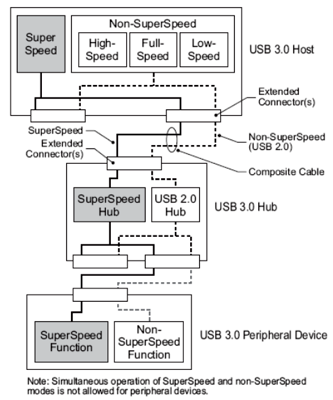
\includegraphics[width=0.6\textwidth]{usb30_architecture}
\caption{USB 3.0 dual-bus architecture (http://www.usb.org/)}
\label{fig:usb30_architecture}
\end{center}
\end{figure}

\begin{figure}[H]
\begin{center}
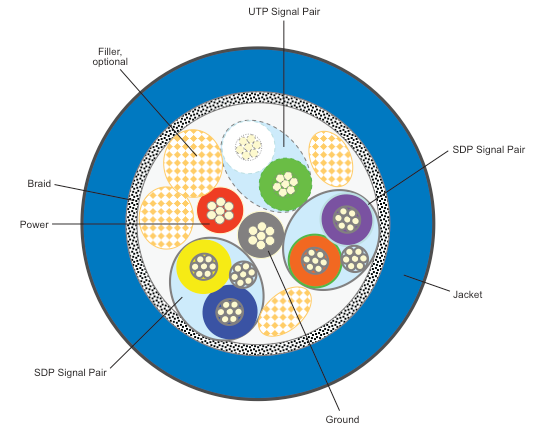
\includegraphics[width=0.6\textwidth]{usb30_cable}
\caption{USB 3.0 cable (http://www.usb3expresscard.com/)}
\label{fig:usb30_cable}
\end{center}
\end{figure}

\section{Comparison with USB 2.0} \label{sec:comparison_with_usb_2.0}

Table \ref{tab:usb_comparison} compares the most important characteristics of USB 3.0 and 2.0, showing the significant differences between the two protocols \cite{AN75705}:

\begin{table}[H]
\begin{center}
\caption{USB 2.0 and 3.0 comparison}
\label{tab:usb_comparison}
\begin{tabu} to \linewidth {|l|X|X|}
\hline
Feature & USB 2.0 & USB 3.0 \\ \hline
Bandwidth & 480 Mbit/s, 12 Mbit/s, 1.5 Mbit/s & 5 Gbit/s, 480 Mbit/s, 12 Mbit/s, 1.5 Mbit/s  \\ \hline
Data interface & Half-duplex over two-wire differential signaling & Dual-simplex over four-wire (twice two-wire) differential signaling; plus USB 2.0 interface for backwards compatibility \\ \hline
Signals (cable) & Four: two for USB 2.0 data, two for VBUS and GND & Ten: four for USB 3.0 data, two for USB 3.0 GND, two for USB 2.0 data, two for VBUS and GND \\ \hline
Bus protocol & Host-directed, polled traffic, packets broadcast to all downstream devices, no multiplexing of data-streams & Host-directed, asynchronous notifications, packets routed to target device only, multiple data-streams for bulk mode possible \\ \hline
Power management & Two modes: Active, Suspend & Four modes: Active (U0), Idle Fast (U1), Idle Slow (U2), Suspend Slow (U3) \\ \hline
Bus power & Low-power device: 100 mA, High-power device: 500 mA & Low-power device: 150 mA, High-power device: 900 mA \\ \hline
Cable length & max. 5 meters & max. ~3 meters (depends on electrical specification) \\ \hline
Data transfer types & Four: Control, Bulk, Interrupt, Isochronous & Four: Control, Bulk, Interrupt, Isochronous \\ \hline
\end{tabu}
\end{center}
\end{table}

\chapter{Cypress FX3} \label{chap:cypress_fx3}

The FX3 \cite{CYUSB3014} is a USB 3.0 micro-controller developed and marketed by Cypress Semiconductor Corporation.
It enables peripherals to be accessed and controlled over USB 3.0, providing the means to easily build USB-enabled devices.
It supports connecting to a wide variety of devices thanks to the several serial buses it implements:

\begin{itemize}
\item I2C master at 100 KHz/400 KHz/1 MHz
\item UART full-duplex
\item SPI master up to 33 MHz
\item I2S master at 32/44.1/48 KHz (mostly audio applications)
\item GPIO general purpose IO pins (partially shared with GPIF2)
\end{itemize}

as well as the flexible, programmable parallel interface GPIF2, which enables data exchange up to 32bit at 100 MHz (400 MByte/s) and allows the implementation of master/slave interfaces common in the industry. Appendix \ref{chap:appendix_clock_frequencies} encloses a list of all clock frequencies and their default values.
A new Direct Memory Access (DMA) engine controls the data transfer between the peripherals, freeing up the processor after initialization for other tasks.
A real-time operating system with support for multiple threads, ThreadX, significantly enhances and simplifies initialization and working with devices, as well as providing a much better and cleaner API to program with.

\section{Comparison with Cypress FX2LP} \label{sec:comparison_with_cypress_fx2lp}

Table \ref{tab:cypress_comparison} compares the most important characteristics of the Cypress FX3 and its predecessor, the Cypress FX2LP, showcasing the relevant differences between the two micro-controllers \cite{AN75705}:

\begin{table}[H]
\begin{center}
\caption{Cypress FX2LP and FX3 comparison}
\label{tab:cypress_comparison}
\begin{tabu} to \linewidth {|l|X|X|}
\hline
Feature & FX2LP & FX3 \\ \hline
USB support & USB 2.0, up to 6 physical endpoints & USB 3.0 and 2.0, USB 2.0 On-The-Go (OTG), battery charging supported, up to 32 physical endpoints \\ \hline
CPU & Enhanced Intel 8051 at 48 MHz & 32-bit ARM926EJ at 200 MHz \\ \hline
SRAM & 16 KB & 512 KB \\ \hline
Boot from & USB, I2C & USB, I2C, SPI, GPIF2 \cite{AN76405} \\ \hline
GPIF & 8/16-bit data bus at 48 MHz & 8/16/32-bit data bus at 100MHz \\ \hline
Peripherals & I2C (up to 400 KHz), UART & I2C (up to 1 MHz), UART, SPI (up to 33 MHz), I2S \\ \hline
Operating System & - & ThreadX RTOS \\ \hline
Compiler / IDE & Keil C for 8051 & Eclipse with GNU ARM tool-chain (GCC) \\ \hline
\end{tabu}
\end{center}
\end{table}

\section{Development Kit} \label{sec:development_kit}

The FX3 development kit \cite{CYUSB3KIT-001} consists of the FX3 development board, shown in Figure \ref{fig:fx3_devboard}, the corresponding USB cable and power adapter, as well as the FX3 Software Development Kit (SDK), detailed in section \ref{sec:development_tools}.
It provides connectivity to all the interfaces that the FX3 micro-controller supports, as well as debugging facilities, and incorporates a 4 Mbit SPI Flash memory. It can load its firmware easily from either USB or the SPI Flash mentioned above, providing for easy testing of new firmware.

\begin{figure}[H]
\begin{center}
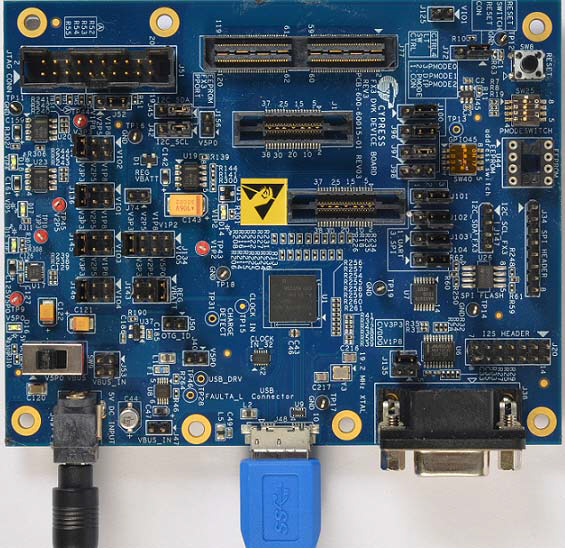
\includegraphics[width=0.5\textwidth]{fx3_devboard}
\caption{FX3 development board (http://www.cypress.com/)}
\label{fig:fx3_devboard}
\end{center}
\end{figure}

\section{Development Tools} \label{sec:development_tools}

The FX3 SDK was completely revamped and features multiple improvements over the SDK for its predecessor, which was based on the Keil C compiler for 8051.

The central development application is now based on the Eclipse IDE, as demonstrated in Figure \ref{fig:fx3_sdk}, and uses the ARM port of the GNU GCC compiler to generate the target binaries. This gives the developer an up-to-date environment in which to work, easily supporting modern features such as auto-completion, multiple projects, integrated API documentation and so on, using a well-known and established interface.

Thanks to a layered, modular approach, developing firmware for the FX3 has become easier and less error-prone. As seen in Figure \ref{fig:fx3_stack}, the user writes his own firmware by leveraging the FX3 firmware framework and its well-documented APIs, which in turn run on the ThreadX real-time operating system. Lots of examples provide a starting point and a kind of documentation on how certain types of problems are to be solved using the FX3 framework. This enables the programmer to focus more on logic and features, than on which bit set to what value to provide some effect, as it was back in the register-driven era of the FX2LP firmware.
High-level APIs are provided to program and setup the USB, GPIF2 and serial (I2C, UART, SPI, I2S, GPIO) interfaces, as well as controlling the DMA engine, how data is exchanged and how to handle USB requests. APIs to access debug facilities as well as the underlying ThreadX RTOS are also provided, as well as advanced APIs to access and control USB and DMA in a much more fine-grained way.
A quick example to illustrate the much cleaner approach possible thanks to the well defined and documented function-based API is shown in Table \ref{tab:cypress_programming}.

\begin{table}[H]
\begin{center}
\caption{Cypress FX3 function-based API versus FX2LP register-driven API}
\label{tab:cypress_programming}
\begin{tabu} to \linewidth {|l|}
\hline
FX2LP \\ \hline
EP0BUF[0] = SETUPDAT[1]; \\
EP0BUF[1]= TIMESTAMP\_MASTER; // PC1 (Port C Pin 1) \\
EP0BCH = 0; \\
EP0BCL = 2; \\
EP0CS \textbar= bmHSNAK; \\ \hline
FX3 \\ \hline
uint8\_t Buffer[2]; \\
Buffer[0] = bRequest; \\
CyU3PGpioGetValue(GPIO\_ID, \&Buffer[1]); // GPIO Pin \\
CyU3PUsbSendEP0Data(2, \&Buffer); \\ \hline
\end{tabu}
\end{center}
\end{table}

Other tools are also included, such as the GPIF2 Designer, which provides an easy way to specify the various characteristics of the GPIF2 interface and its programmable states, using a simple graphical user interface; or the ControlCenter application, which enables easy uploading and flashing of new firmware to the FX3 for testing purposes.

The FX3 firmware is now generated in only one format directly by the tool-chain, and this format can then be uploaded directly to the micro-controller or to a memory device from which it can later read it and boot from. No multiple formats or conversions between them (BIX, HEX, IIC formats) are needed anymore.
Several examples, guides, various documentation, as well as an auto-update feature for the SDK complete the offering.

\begin{figure}[h]
\begin{center}
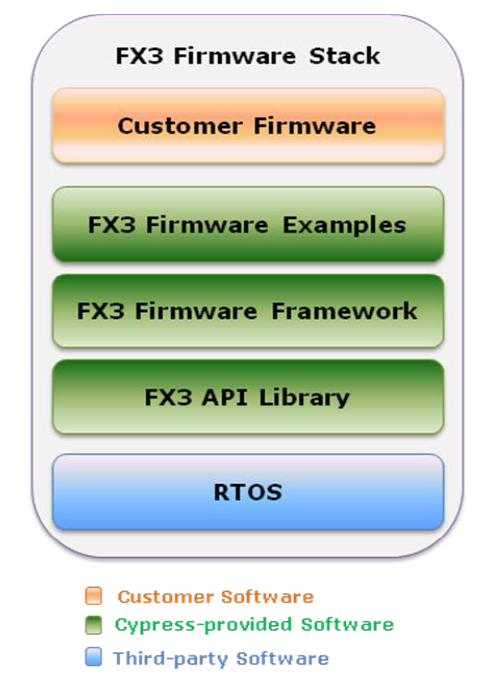
\includegraphics[width=0.4\textwidth]{fx3_stack}
\caption{FX3 firmware stack (http://www.cypress.com/)}
\label{fig:fx3_stack}
\end{center}
\end{figure}

\begin{figure}[h]
\begin{center}
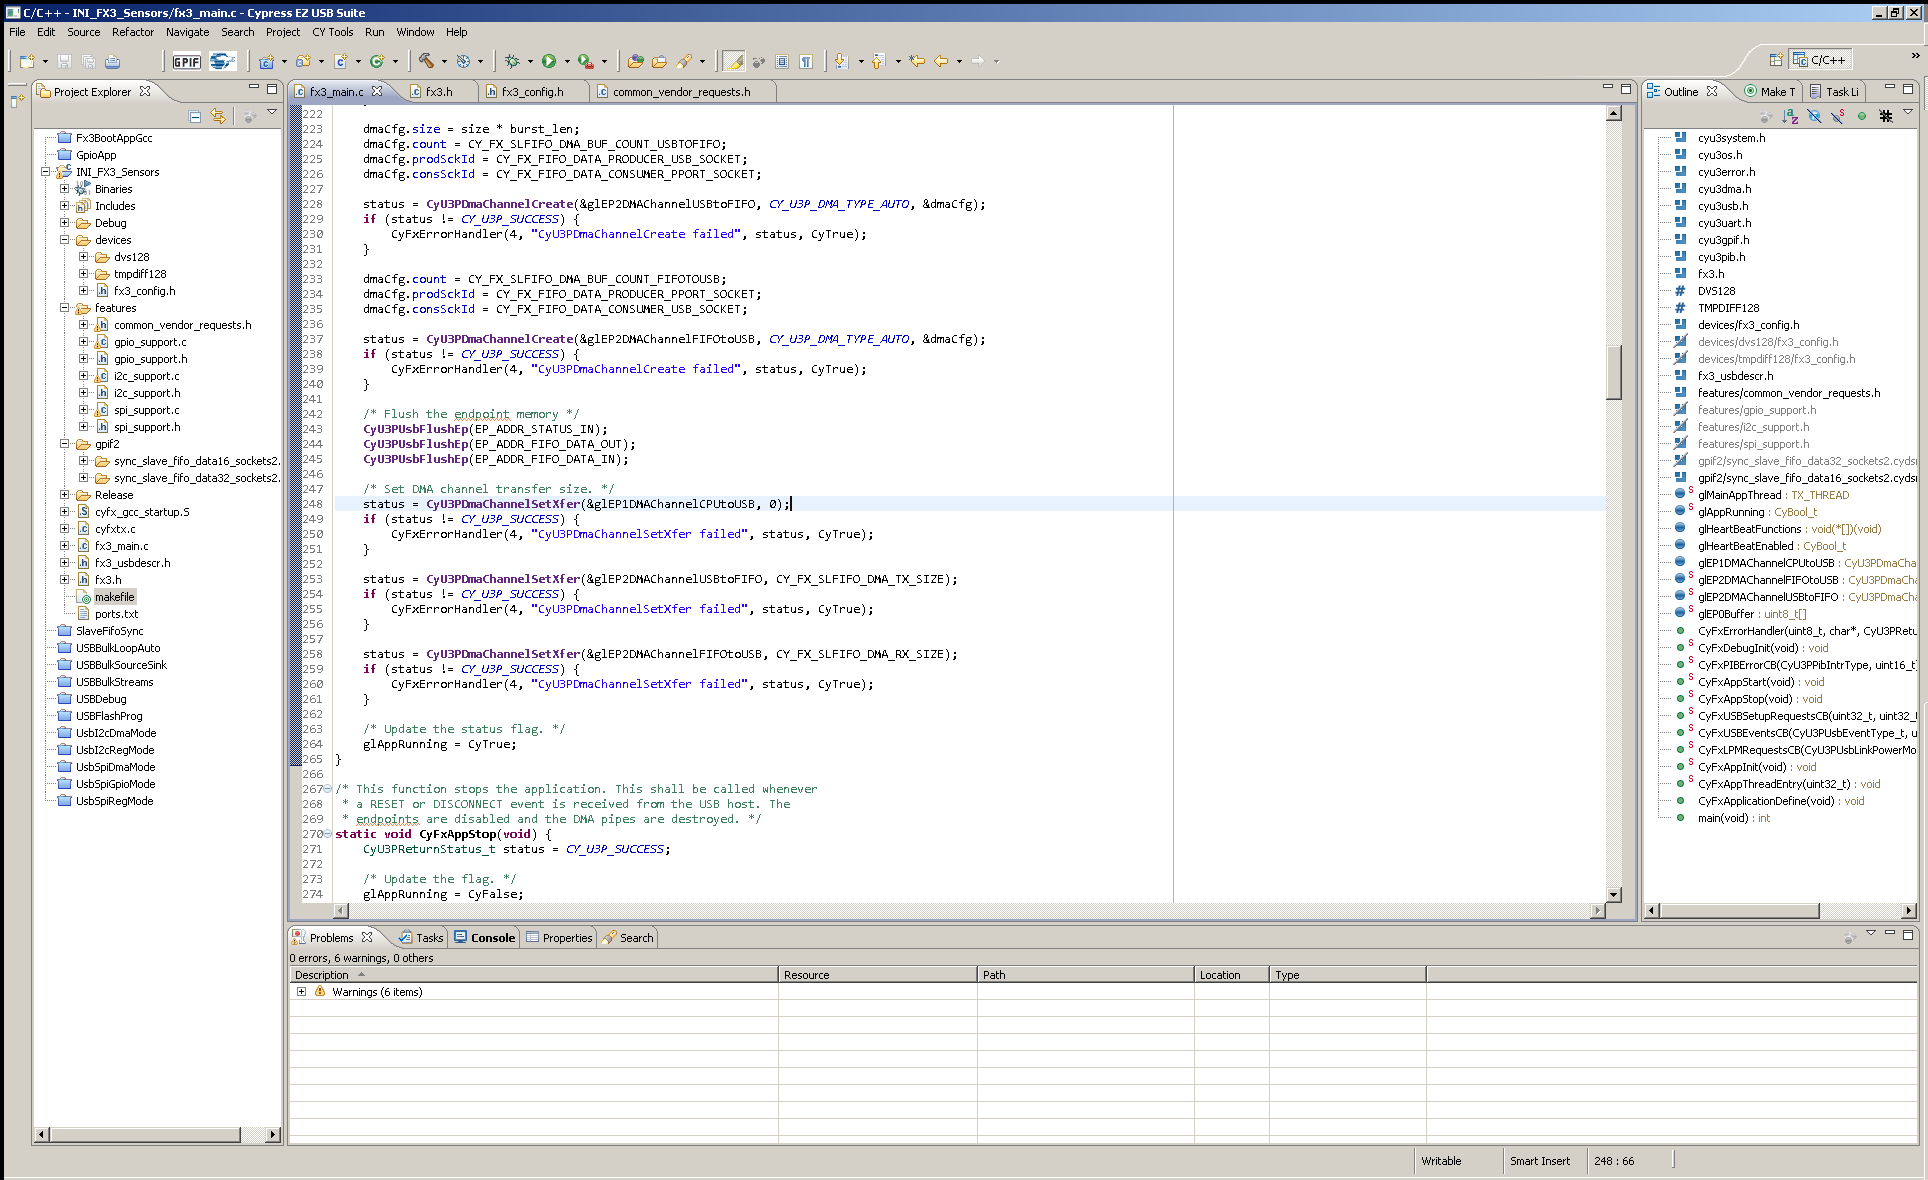
\includegraphics[width=0.55\textwidth]{fx3_sdk}
\caption{FX3 Eclipse-based SDK}
\label{fig:fx3_sdk}
\end{center}
\end{figure}

\chapter{FX3 Firmware} \label{chap:fx3_firmware}

The firmware for the FX3 is a complete re-development. It would have been difficult \cite{AN76348} to port the old FX2 firmware in a straight-forward manner, since everything changed so radically, from the possibilities that the hardware offers, to the way it's programmed and the tools used. Further, as explained below, a re-engineering effort was desirable. As such, the old firmware was just used as a place to gather the requirements that a new, general-purpose firmware would need to satisfy at the very least, and the new firmware is based upon a completely new architecture and new code.

\section{Comparison with FX2 Firmware} \label{sec:comparison_with_fx2_firmware}

When looking at the FX2 firmware, it became quickly evident, as shown in Figure \ref{fig:fx2_multiple}, that it had suffered major fragmentation during its life-cycle; indeed about 14 different firmware projects exist currently for almost the same number of sensor devices and variants thereof. Most of those consist of an older version of the working firmware being copied and some code here and there being adjusted to the new requirements of the device currently being worked on. This approach to software development is sub-optimal, as it heavily splits the effort and doesn't provide for a common way to maintain the older code bases, due to heavy code duplication, making it even more difficult to understand and compare the functionality of the various FX2 firmware implementations.

To remedy the above situation, it was decided to write not one firmware for each device in the case of the FX3, but instead a firmware framework, offering common, as well as optional, functionality in a well-defined way, and then enable each new device to simply be a new set of configuration files to control the framework's behavior, enable functionality as needed and, depending on the application, hook into certain parts of the framework and supply device-specific code-paths for certain tasks.

\begin{figure}[h]
\begin{center}
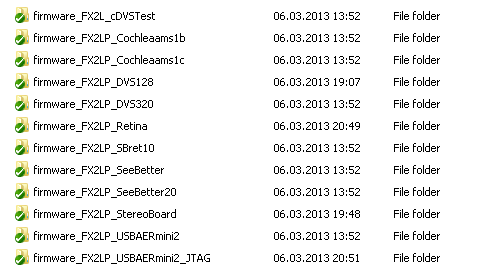
\includegraphics[width=0.8\textwidth]{fx2_multiple}
\caption{Multitude of FX2 firmware projects}
\label{fig:fx2_multiple}
\end{center}
\end{figure}

\section{Architecture} \label{sec:architecture}

The core concepts of the new architecture are: small common core; additional functionality as optional, separate modules; and per-device configuration and customization.
The minimal core is composed of the device initialization and configuration code, as well as the configuration for the GPIF2 interface to exchange data, either 16 or 32 bits at a time, on an USB end-point (\ref{sec:slave_fifo_interface_data_end-point}). An additional USB end-point provides status data exchange (\ref{sec:debugging_status_end-point}). Optionally, one can enable communication over various serial protocols, such as I2C (\ref{sec:i2c_bus}), SPI (\ref{sec:spi_bus}) and GPIO (\ref{sec:gpio}). I2S and UART were not taken into consideration, as no present or future sensor presented any use case for them. All of this is configured per-device, using a mixture of \#defines, functions and arrays, enabling high flexibility in the deployment of customized firmware. The following sections will explore each feature in higher detail.
Three USB end-points are provided: EP 0, the control end-point, is responsible for managing vendor requests, which can be seen as the commands a USB device can react and respond to. This end-point is always present, and actually mandated by the protocol standard. EP1, the status end-point, and EP2, the data end-point, will be explained in detail in sections \ref{sec:debugging_status_end-point} and \ref{sec:slave_fifo_interface_data_end-point}.

\section{File Structure} \label{sec:file_structure}

Let's go over each file and directory in the new structure, as seen in Figure \ref{fig:fx3_fw_structure} in more detail:

\begin{itemize}
\item{cyfx\_gcc\_startup.S} is an assembly file provided by Cypress, which has to be part of any firmware project and should never be touched by the user. It initializes the device and jumps to the user-supplied initialization code.
\item{cyfxtx.c} is another file provided by Cypress, containing parts of the API the user is going to have access to later, mostly concerning memory management. It can be edited if particular memory management requirements have to be met.
\item{fx3.h} is the main configuration file for global settings. Several framework-wide settings can be changed here in the form of \#defines, such as the default log level, the default thread stack-sizes and priorities, as well as all USB end-point and DMA settings. Several helper macros for general usage, as well as several global variables, are also declared here as to be accessible everywhere; like the global error handler or the KILO/MEGA macros for improved readability. All of these settings can also be tweaked on a per-device basis.
\item{fx3\_main.c} includes the main firmware functionality. It is responsible for initializing the device according to the configuration, for creating the various threads that will handle requests, and initializing the various configured serial and USB sub-systems. It further provides the global error handler, as well as brings up the USB end-points for data exchange. Most of the above is usually done by calling out to the appropriate functions implemented within the feature or device-specific modules.
\item{fx3\_usbdescr.h} contains a series of C-structs, which represent the various USB descriptors of the device. USB descriptors are pieces of information that the host system uses to discover what abilities, services and features the connected device has to offer, such as the maximum USB version supported, or how much electrical current is needed, or who the manufacturer of the device is. The most important settings, such as the Vendor ID or Product ID, can be overridden per-device.
\item{gpif2 directory} contains the configuration files for the GPIF2 interface, once for data exchange of 16 bits per clock cycle (the default setting), and once for 32 bits per cycle. Both configurations were generated using the GPIF2 Designer tool from Cypress.
\item{features directory} contains the implementation of the various additional features, so as to keep them well separated from the core. The header files present usually define which vendor requests are supported by the module in question and which functions are exported and visible to other modules.
\item{features/common\_vendor\_requests.{h,c}} handles several general-purpose vendor requests, ranging from status information to debugging helpers. See section \ref{sec:common_vendor_requests} for a more detailed explanation.
\item{features/gpio\_support.{h,c}} implements the handling of General-Purpose I/O (GPIO) pins, as well as their initial configuration. Section \ref{sec:gpio} contains more information on all supported modes.
\item{features/heartbeat.{h,c}} contains the heartbeat system, which enables the execution of defined functions at timed intervals to accomplish some task, such as flashing a LED. Section \ref{sec:heartbeat} enters into more detail.
\item{features/i2c\_support.{h,c}} enables the firmware to support the I2C serial bus to exchange data with connected peripheral devices. Section \ref{sec:i2c_bus} has a detailed explanation of the protocol and the involved code.
\item{features/spi\_support.{h,c}} handles support for the SPI bus, another serial data bus with slightly different characteristics than I2C and higher speeds. See section \ref{sec:spi_bus} for details.
\item{devices directory} contains the device-specific configuration, which makes this firmware so flexible and powerful.
\item{devices/fx3\_select.h} lists all supported devices, and selects the one for which the firmware should be compiled at this moment in time.
\item{devices/fx3\_config.h} holds all the \#defines and function declarations for the various optional features and configuration settings, that have to be set and implemented by a device to enable certain functionality.
\item{devices/\$device/\$device\_config.h} contains the per-device \#defines.
\item{devices/\$device/\$device\_config.c}, on the other hand, contains the per-device function implementations and array definitions, as required by the enabled features.
\end{itemize}

\begin{figure}[H]
\begin{center}
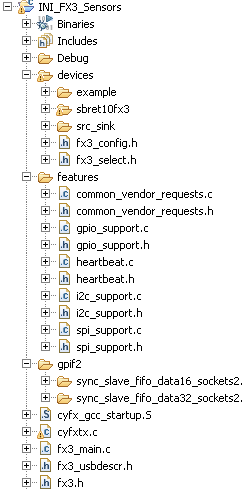
\includegraphics[width=0.45\textwidth]{fx3_fw_structure}
\caption{FX3 firmware structure}
\label{fig:fx3_fw_structure}
\end{center}
\end{figure}

\section{Debugging and Status End-Point} \label{sec:debugging_status_end-point}

The status end-point, EP1, is a special end-point meant for quick notifications to be sent out from the device to the host. As such, it only operates in that one direction (from FX3 to USB), and can only send data packets of up to 64 bytes. These limitations are imposed by the fact that this is an INTERRUPT type end-point, which, on the other hand, offers guaranteed latency, which is of critical importance for being able to send status messages in a timely manner.

On top of the status-endpoint, the standard debug facility is implemented, enabling easy status and error messages to be sent in a common format. The following function is responsible for sending error messages; it expects a valid log level (see section \ref{sec:common_vendor_requests}, VR\_LOG\_LEVEL), as well as a message explaining the problem and an appropriate error code.

\begin{lstlisting}
void CyFxErrorHandler(uint8_t log_level, const char *debug_message, CyU3PReturnStatus_t error_code);
\end{lstlisting}

The format of the sent message is as follows:

\begin{table}[H]
\begin{center}
\caption{Error message format}
\label{tab:error_message_format}
\begin{tabu} to \linewidth {|l|l|}
\hline
Byte & Content \\ \hline
0 & 0x00, which signifies a standard error message \\ \hline
1 & the error code \\ \hline
2-5 & the current time-stamp \\ \hline
6-63 & the error message, up to 58 characters (64 maximum minus 6) \\ \hline
\end{tabu}
\end{center}
\end{table}

It can happen that a message is not delivered to the host, because, to avoid blocking the handler threads, the logging function returns right away. If, when it is called, no buffers are free to receive the new log message, because their number is limited and they could have already been consumed by other messages that haven't yet been delivered to the host either, the message will be dropped. The occurrence of such drops is counted and can be queried with the VR\_STATUS vendor request. In practice this rarely happens, unless a veritable storm of errors is produced, while the device is running and communicating; but is more easily possible if the device is running, but not connected to USB. In such a case, only the first few messages are preserved for later sending over USB when the device is again connected, any successive ones are lost.

\section{Slave FIFO Interface and Data End-Point} \label{sec:slave_fifo_interface_data_end-point}

For data transfers, the data end-point is provided. EP2 is a BULK type end-point, which is perfect for streaming large amounts of data. It is directly linked to the GPIF2 interface, and is used for high-speed data exchange between the external device connected to the GPIF2 interface and USB.
The GPIF2 interface's default configuration is that of a 16 bit bi-directional Slave FIFO, meaning it can transfer data to and from the external device, in FIFO order, and it's the device that initiates read or write cycles, not the FX3 micro-controller. The FX3 provides a series of buffers onto which data is written to or read from, and several status flags so that the external device knows when it can access the FX3 for those operations and when not. Those four flags signal if the currently selected buffer is either FULL, ALMOST\_FULL, ALMOST\_EMPTY or EMPTY. Please refer to \cite{AN65974} for more detailed information, especially on how external devices access the buffer and the required timings thereof.
Through configuration (\#define GPIF\_32BIT\_SUPPORT\_ENABLED), it is possible to switch to a 32 bit wide data exchange, but sacrificing at the same time sixteen of the limited GPIO pins to provide for the needed additional data lines.

\section{Custom DMA Processing} \label{sec:custom_dma_processing}

Normally, data packets are forwarded quickly and directly from the external interfaces to USB and vice versa, thanks to the DMA engine. It is though possible to bypass this mechanism to gain greater control over the data packets in transit, and being then able to examine them, modify them or discard them directly on the FX3's ARM CPU, by deviating the data flow in question through it. Support for this functionality is provided by the following \#defines and functions:

\begin{lstlisting}
#define DMA_USBTOFX3_CALLBACK (0)

void CyFxDmaUSBtoFX3Callback(CyU3PDmaChannel *chHandle, CyU3PDmaCbType_t type, CyU3PDmaCBInput_t *input);

void CyFxDmaUSBtoFX3CallbackInit(CyU3PDmaChannel *chHandle);
void CyFxDmaUSBtoFX3CallbackDestroy(CyU3PDmaChannel *chHandle);

#define DMA_FX3TOUSB_CALLBACK (0)

void CyFxDmaFX3toUSBCallback(CyU3PDmaChannel *chHandle, CyU3PDmaCbType_t type, CyU3PDmaCBInput_t *input);

void CyFxDmaFX3toUSBCallbackInit(CyU3PDmaChannel *chHandle);
void CyFxDmaFX3toUSBCallbackDestroy(CyU3PDmaChannel *chHandle);
\end{lstlisting}

As you can see, it is possible to enable the functionality for the IN and OUT channels separately. The user is expected to implement a main function to manipulate the data packets moving over the specified DMA channel, as well as two helper functions that are called when the DMA channel is either initialized or destroyed.
Please use this feature sparingly, as having to move the high-speed data streams from EP2 through the CPU adds a heavy load to it and slows down the data transfer. The more complex the inspection and algorithms being applied on the data, the higher the slow-down will be; keep in mind, this is only a 200 MHz RISC CPU.

\section{Common Vendor Requests} \label{sec:common_vendor_requests}

USB vendor requests are used to send commands to USB devices, always over end-point zero, and have a well defined format \cite{USB_Nutshell}; the setup packet consisting of eight bytes, with the following meaning: byte 0 encodes the direction of the data transfer, as well as its type and the intended recipient (usually the device); byte 1 contains the code of the USB request (bRequest field), bytes 2-3 represent the wValue field, containing any 16 bit value; bytes 4-5 contain the wIndex field, again with 16 bits of user-defined information; and lastly, bytes 6-7 contain the wLength field, which specifies the length of the data portion to come afterwards. In other words, one can have a few hundred commands per device (the 0x00 to 0x3F codes are reserved), each of which can be supplied up to 32 bits of data to configure their behavior (wValue plus wIndex fields), to then transfer up to 65 KB of data to the device or from it, in a single request. All vendor requests supported by this firmware are listed in Appendix \ref{chap:appendix_vr_assignment}.

The common vendor requests module supports general purpose functionality, concerning itself with device information and debugging. All vendor requests that can't be handled by a module, because they are not recognized, are forwarded to the next, until either a module is found which is able to handle the specified request, or an error is sent back to the user.

The VR\_MS\_FEATURE\_DSCR vendor request provides an implementation for the WCID feature offered by the Microsoft Windows WinUSB driver, which allows a device to specify that it is compatible with and wants the WinUSB driver to be responsible on the host-side for communication, freeing the consumer from having to worry about driver installation and offering a well tested and solid way to exchange data. This is done by having the device supply a particular USB descriptor, which in turn specifies a particular vendor request that the Windows USB sub-system will then execute to query the needed information from the device. The format of the response is defined by Microsoft documentation, and consists of 40 bytes containing various pieces of data about the device and how it can interact with the Windows USB sub-system. This request is never initiated by users of the device themselves, and support for it has to be explicitly enabled in the device configuration with the MS\_FEATURE\_DESCRIP
 TOR\_ENABLED \#define.

VR\_TEST implements a quick and simple way to test the device: any message sent along with it, is then sent back over the status end-point, giving an easy way to test communication in both directions over different end-points. Only the first 58 bytes are sent back, as that's the limit of external data the status end-point can send in one go (see section \ref{sec:debugging_status_end-point} for a more detailed explanation on why this is so).

The VR\_LOG\_LEVEL request sets the default log level, delimiting which log messages generated by the firmware are sent out over the status end-point to the host. The wValue field encodes one of the following supported values:

\begin{table}[H]
\begin{center}
\caption{Supported log levels}
\label{tab:log_levels}
\begin{tabu} to \linewidth {|l|c|}
\hline
Log Level & Value \\ \hline
LOG\_EMERGENCY & 0 \\ \hline
LOG\_ALERT & 1 \\ \hline
LOG\_CRITICAL & 2 \\ \hline
LOG\_ERROR & 3 \\ \hline
LOG\_WARNING & 4 \\ \hline
LOG\_NOTICE & 5 \\ \hline
LOG\_INFO & \textbf{6} \\ \hline
LOG\_DEBUG & 7 \\ \hline
\end{tabu}
\end{center}
\end{table}

The default value is set in fx3.h to LOG\_INFO. Further, setting the value to LOG\_DEBUG, will also enable a heart-beat message to be sent over the status end-point every five seconds approximately.

The VR\_FX3\_RESET command simply hard-resets the device.

VR\_STATUS sends back some information on the run-time firmware status. Its returned message currently consists of eight bytes, divided as follows:

\begin{table}[H]
\begin{center}
\caption{VR\_STATUS response format}
\label{tab:vr_status_response_format}
\begin{tabu} to \linewidth {|l|l|}
\hline
Byte & Content \\ \hline
0-3 & the current time-stamp \\ \hline
4 & whether the application is running (end-points successfully enabled or not) \\ \hline
5 & the currently set log level \\ \hline
6 & the number of log messages that could not be delivered \\ \hline
7 & the current USB connection speed \\ \hline
\end{tabu}
\end{center}
\end{table}

VR\_SUPPORTED instead contains information about some of the compile-time flags that influence which optional features are available. It currently consists of the following seven bytes:

\begin{table}[H]
\begin{center}
\caption{VR\_SUPPORTED response format}
\label{tab:vr_supported_response_format}
\begin{tabu} to \linewidth {|l|l|}
\hline
Byte & Content \\ \hline
0 & 32 bit GPIF2 interface enabled instead of 16 bit \\ \hline
1 & I2C support enabled \\ \hline
2 & SPI support enabled \\ \hline
3 & GPIO support enabled \\ \hline
4 & Custom Vendor Requests defined \\ \hline
5 & Custom DMA processing defined on the IN path (from USB to FX3) \\ \hline
6 & Custom DMA processing defined on the OUT path (from FX3 to USB) \\ \hline
\end{tabu}
\end{center}
\end{table}

\section{Custom Vendor Requests} \label{sec:custom_vendor_requests}

It is possible to add new, custom vendor requests for each different device, so as to provide support for specific features or react differently to certain requests. This can be achieved by specifying a particular handler function, whose signature is shown below, that then receives all the relevant information about the request being handled, as well as enabling the appropriate \#define. It is the first vendor request handler being called, and can as such also override the common vendor requests from section \ref{sec:common_vendor_requests} if so desired, though it is highly discouraged.
All useful vendor request information is passed along to the function, already split up, and the glEP0Buffer global buffer can be used to read or write data with the appropriate functions.

\begin{lstlisting}
#define DEVICE_SPECIFIC_VENDOR_REQUESTS (0)

CyBool_t CyFxHandleCustomVR_DeviceSpecific(uint8_t bDirection, uint8_t bRequest, uint16_t wValue, uint16_t wIndex, uint16_t wLength);
\end{lstlisting}

\section{GPIO} \label{sec:gpio}

Support for General-Purpose Input/Output (GPIO) control represents the backbone of controlling external hardware, by giving fine-grained control over several pins and wires: the current value can either be sensed (input), or set to on/off (output), for specified periods of time. This is used to send or receive single bits of information to connected peripherals, such as controlling LEDs, or resetting an external sensor, or reacting to some interrupt from outside.
The VR\_GPIO\_GET and VR\_GPIO\_SET vendor requests are responsible for, respectively, reading the current value of a GPIO pin and setting the value to something supplied by the user.
The GET request simply expects the wValue field to be set to the ID of the GPIO one wants to query, and sends back one byte containing the current status.
The SET request also expects the wValue field to contain the GPIO ID, but further accepts various modes to be passed through the wIndex field:

\begin{table}[H]
\begin{center}
\caption{VR\_GPIO\_SET modes}
\label{tab:vr_gpio_set_modes}
\begin{tabu} to \linewidth {|l|l|X|}
\hline
Value & Mode & Description \\ \hline
0 & OFF & turns the specified GPIO off \\ \hline
1 & ON & turns the specified GPIO on \\ \hline
2 & TOGGLE & turns the specified GPIO on and off again \\ \hline
3 & TIMED & turns the specified GPIO on, waits for the amount of time (in milliseconds) specified in the first two bytes of the data portion (in network order), then turns it off again\\ \hline
4 & RECURRING & sets up a timed, recurring GPIO switch; the first two bytes of the data portion (in network order) specify the time in milliseconds between on/off cycles. Useful for flashing LEDs or resetting timers. See the heartbeat documentation in section \ref{sec:heartbeat} to understand the limitations of the timer used for this.\\ \hline
\end{tabu}
\end{center}
\end{table}

A list of which GPIO IDs \cite{CYUSB3014} are available depending on the configuration can be found in Appendix \ref{chap:appendix_pin_assignment}. All requests are checked internally against this list, so it's impossible to set invalid GPIO pins via USB vendor requests.
GPIO support needs to be enabled in the device configuration, and an initial configuration has to be supplied, so that the firmware can know which GPIO pins are used in which mode, and then initialize them appropriately, and later check that accesses to them are valid. As shown with the following code, GPIO configuration consists of an array of small structs, each containing a valid GPIO ID and the corresponding type setting (refer to table \ref{tab:gpio_configuration_types} for a list of all possible type settings). Further, the length of the array has to be supplied in the appropriately named variable. The configuration array is meticulously checked for invalid values at start-up and the firmware refuses to boot if any misconfiguration is detected. The values must be those indicated in the valid GPIO list, there can be no duplicates, and the types must be correct.

\begin{lstlisting}
#define GPIO_SUPPORT_ENABLED (0)

typedef struct {
    const uint8_t gpioId;
    const uint8_t gpioType;
} gpioConfig_DeviceSpecific_Type;

extern gpioConfig_DeviceSpecific_Type gpioConfig_DeviceSpecific[];
extern const uint8_t gpioConfig_DeviceSpecific_Length;

void CyFxHandleCustomGPIO_DeviceSpecific(uint8_t gpioId);

#define GPIO_DEBUG_LED_ENABLED (0)
#define GPIO_DEBUG_LED_NUMBER (0xFF)
\end{lstlisting}

For interrupt type GPIOs (up to 24 of them can be configured as such), the CyFxHandleCustomGPIO\_DeviceSpecific() function has to be defined: each time an interrupt is detected on an appropriately configured input GPIO, this function gets called and the ID of the GPIO that generated the event is supplied. The user can then react to it inside that function in any way he sees fit, since, through a mechanism called event-flags, the function is called from the main firmware thread, and not from the internal interrupt handler, which would not have provided any useful access to send data over USB etc. from inside the restricted interrupt handler context.

It is further possible to enable and specify a GPIO ID as a debug LED, it will then be toggled every time an error message is sent over the status end-point. This GPIO has to be configured as an output before-hand.

Another useful feature that was implemented is automatic transformation of active high and low signals. Electrical signals represent bits by their voltage: a low voltage represents 0 and a high voltage represents 1. This is called an active-high signal: the 1 is the high voltage. Many devices on the other hand work with or expect also active-low signals: the meaning is inverted, and the logical 1 is represented by the low voltage. To free the user from having to manually figure out what each signal needs to be set to in order for it to be active, the GPIO configuration abstracts the concept of voltage away and the user simply has to know that ON means logical 1 and OFF means logical 0. The firmware converts the values automatically internally, thanks to the supplied initial GPIO configuration's type setting: if the type is written in upper-case, it means the GPIO in question shall be active-high, if the type is written in lower-case, it shall be active-low. Once this initial configur
 ation is done, the user doesn't have to care about voltage meanings anymore, but can simply work with the logical meaning of the signals (ON/OFF), trusting that the firmware will do the right conversions.

\begin{table}[H]
\begin{center}
\caption{GPIO configuration: types}
\label{tab:gpio_configuration_types}
\begin{tabu} to \linewidth {|l|l|}
\hline
Value & Description \\ \hline
'O', 'o' & simple output (has to be set manually) \\ \hline
'I', 'i' & simple input (has be queried manually) \\ \hline
'P', 'p' & pos-edge interrupt, triggers every time the GPIO transitions from OFF to ON \\ \hline
'N', 'n' & neg-edge interrupt, triggers every time the GPIO transitions from ON to OFF \\ \hline
'B', 'b' & both-edge interrupt, triggers on both pos-edge and neg-edge transitions \\ \hline
'L', 'l' & low interrupt, triggers when the GPIO is in OFF state \\ \hline
'H', 'h' & high interrupt, triggers when the GPIO is in ON state \\ \hline
\end{tabu}
\end{center}
\end{table}

\section{Heartbeat} \label{sec:heartbeat}

The heartbeat system provides a general framework for executing functions at defined time intervals. This was developed as a general solution to implement flashing LEDs or keep-alive messages, for which it is currently used in the firmware.
Two functions enable the programmer to add or remove functions, with a 32 bit input argument, from the heartbeat system. When adding a function, a 16 bit value specifies the time interval in milliseconds between calls to the function. For performance and resource consumption reasons, the interval will be converted to the nearest multiple of 512 internally, so about 0.5 seconds of precision are given, called timer ticks (one timer tick = 512 milliseconds). This functionality is intended for long running, repeating tasks, and not for hard-real-time tasks or tasks which require a high degree of precision in the timer.

\begin{lstlisting}
CyU3PReturnStatus_t CyFxHeartbeatFunctionAdd(void (*func)(uint32_t input), uint32_t input, uint16_t timer);
void CyFxHeartbeatFunctionRemove(void (*func)(uint32_t input), uint32_t input);
\end{lstlisting}

\section{I2C Bus} \label{sec:i2c_bus}

Inter-Integrated Circuit (I2C) is a serial data bus invented by Philips in the eighties and standardized in the nineties. It provides support for multiple master devices addressing several slave devices over a two wire bus. The two wires are Serial Data (SDA) and Serial Clock (SCL), the clock can run at 100 KHz, 400 KHz or 1 MHz. In the case of the FX3 I2C support, only one master can be present: the FX3 itself. Slave devices are usually selected with a 7 bit address, meaning that up to 128 different devices could be connected to the bus theoretically. The master initiates communication by sending a START bit, followed by the 7 bit address, followed by 1 bit indicating whether it wants to read (1) or write (0). If the indicated slave exists, it will respond with an ACK bit, and the two will then exchange data as indicated.

To easily support the configuration of multiple devices, the firmware requires an array of structs to be populated with the relevant information on the connected slave devices. As most I2C devices are either EEPROMs or provide an EEPROM-like interface for sending commands and reading/writing data, special support was included to simplify working with them, by being able to specify the length of the memory address that's sent to the device, the page size for optimal performance, and the total memory size of the device.
In detail, the required information consists of the slave's address (7 lower bits, MSB has to be zero), the length in bytes of the memory address, the page size (which has to be a multiple of two) and the total size of the device, again both in bytes, as well as the maximum frequency in Hertz the device can operate on. This last piece of data is used to compute the highest common frequency at which all devices connected to the bus can operate, which is then used as default \ref{chap:appendix_clock_frequencies}.

\begin{lstlisting}
#define I2C_SUPPORT_ENABLED (0)

typedef struct {
    const uint8_t deviceAddress;
    uint8_t addressLength;
    uint16_t pageSize;
    const uint32_t deviceSize;
    const uint32_t maxFrequency;
} i2cConfig_DeviceSpecific_Type;

extern i2cConfig_DeviceSpecific_Type i2cConfig_DeviceSpecific[];
extern const uint8_t i2cConfig_DeviceSpecific_Length;
\end{lstlisting}

On the USB side, two vendor requests are provided to interact with I2C devices from the host: VR\_I2C\_CONFIG and VR\_I2C\_TRANSFER.
The configuration request sets up all necessary parameters for the subsequent transfer requests, enabling several checks to be done on them to guarantee correctness and performance. The lower byte of wValue contains the address of the device to talk to, the upper byte specifies the  length in bytes of the memory address that can be supplied later on in transfer calls (maximum length is four bytes, zero means to not change the default value coming from the configuration array above). The wIndex field contains the 16 bit page-size value, which has to either be a power of two (up to the maximum transfer size, usually 4096 bytes), or zero for no change. Usually, if the configuration array above was filled correctly, the latter two values should always be zero.

The VR\_I2C\_TRANSFER request performs either a read or a write from the configured I2C device \cite{RM-MPU-6000A}, depending on its direction. The wValue and wIndex fields are concatenated to form a memory address of up to 32 bits (upper 16 bits wValue, lower 16 bits wIndex), from which up to wLength bytes of data are going to be either read or written. As already mentioned, particularities of EEPROM memory such as how to split a big request into appropriate pieces to take advantage of the memory's page-size alignment, or the length or format of the I2C commands to request a read or write at a particular address, are automatically taken care of by the firmware.

\section{SPI Bus} \label{sec:spi_bus}

The Serial Peripheral Interface (SPI) bus is a synchronous serial bus that is able to operate in full-duplex mode. It follows the master/slave model, where the master initiates the data exchange with the slave. Multiple slaves are supported by providing multiple slave-select lines, that can be toggled to enable a particular slave to receive commands. The standard implementation consists of four wires: Serial Clock (SCLK, from master), Master Output/Slave Input (MOSI, from master), Master Input/Slave Output (MISO, from slave) and Slave Select (SS, from master). No explicit address is used as it was with I2C to select a slave, but instead a slave device is selected by toggling its SS line. The higher frequency of up to 100 MHz enables much faster data exchange than is possible with I2C, as well as full-duplex exchange, albeit by using more wires (four, plus one more for each additional slave in the simplest configuration). The FX3 supports being a SPI master at frequencies up to 33 MHz
  and provides out-of-the-box support for one SS line and thus one connected slave device, using the provided SPI access API.

Given the above advantages of the SPI bus, it is often used in the industry, especially for accessing Flash memory, or for sending configuration to FPGAs, both of which are concrete use cases for the firmware presented here. Like I2C, SPI is an optional feature that has to be enabled and configured, again by supplying an array of structs that contain the needed information about connected SPI devices. The device address field here contains either a zero to indicate to use the default SS line, or a valid GPIO ID that can be used for additional SS lines if multiple devices are to be supported. The default SS line has to always be used (else we'd be wasting a pin!), and the additional GPIO IDs can't be used or configured in the GPIO sub-system, to avoid interference between the two. Of course, no duplicates are allowed either. The address length, page-size and device size fields have the same meaning and format as the I2C ones (see section \ref{sec:i2c_bus}), as they are used for the sa
 me special, enhanced handling of read/write requests to memory-like devices. The maxFrequency field specifies the maximum frequency in Hertz at which the device in question can operate, so that the bus can be set to the highest common frequency supported by all devices \ref{chap:appendix_clock_frequencies}. The SSPolarity field indicates the polarity of the SS line: TRUE means active-high, FALSE active-low.

\begin{lstlisting}
#define SPI_SUPPORT_ENABLED (0)

typedef struct {
    const uint8_t deviceAddress;
    uint8_t addressLength;
    uint16_t pageSize;
    const uint32_t deviceSize;
    const uint32_t maxFrequency;
    const CyBool_t SSPolarity;
} spiConfig_DeviceSpecific_Type;

extern spiConfig_DeviceSpecific_Type spiConfig_DeviceSpecific[];
extern const uint8_t spiConfig_DeviceSpecific_Length;
\end{lstlisting}

Four USB vendor requests are provided to interact with SPI devices.
VR\_SPI\_CONFIG is similar to the I2C configuration command, it sets up all necessary parameters for the subsequent transfer requests, enabling several checks to be done on them to guarantee performance and correctness. The lower byte of wValue contains the address of the device to talk to (its SS line), the upper byte specifies the  length in bytes of the memory address that can be supplied later on in transfer calls (maximum length is four bytes, zero means to not change the default value coming from the configuration array above). The wIndex field contains the 16 bit page-size value, which has to either be a power of two (up to the maximum transfer size, usually 4096 bytes), or zero for no change. Further, up to wLength provided bytes of data (up to a maximum of 256) are stored so as to support arbitrary length SPI command sequences to be sent, for devices which do not follow memory-device like conventions.

The VR\_SPI\_CMD request enables arbitrary commands to be sent to an SPI device \cite{TN1222}. If any command was previously set with the VR\_SPI\_CONFIG request, it will be sent to the device, accompanied by either writing the data sent with this request (wLength bytes), or reading up to wLength bytes back from the device. It is both possible to inhibit the sending of the command by setting the wIndex field to one, or to inhibit the sending of any additional data by setting wLength to zero. This enables sending commands without any subsequent data, or one command, followed by multiple data requests, for example in case the size of the data to be transmitted exceeds 65 KB. The type of the request, read or write, is determined by its direction.

VR\_SPI\_TRANSFER was specifically created to ease handling of SPI Flash memory devices \cite{W25Q80BW}, which offer higher storage capabilities than I2C EEPROMs at higher transfer rates, and are usually preferred for storing data, such as the firmware itself, to enable the device to boot on its own.
It performs either a read or a write from the SPI device, depending on its direction. The wValue and wIndex fields are concatenated to form a memory address of up to 32 bits (upper 16 bits wValue, lower 16 bits wIndex), from which up to wLength bytes of data is going to be either read or written as directed. Particularities of Flash memory such as how to split a big request into appropriate pieces to take advantage of the memory's page-size alignment, or the length or format of the common SPI commands to request a read or write at a particular address from Flash memory, are automatically taken care of by the firmware. Also protocol details such as sending write-enable commands before any write and selecting/deselecting the SS line are taken care of internally.

VR\_SPI\_ERASE is another, complementary request to VR\_SPI\_TRANSFER, specifically for Flash memory devices. A Flash memory device needs to be erased before it can be written to, and this erasing is always done in big chunks (blocks) of memory, for performance reasons. The wValue and wIndex fields are concatenated to form a memory address of up to 32 bits (upper 16 bits wValue, lower 16 bits wIndex), at which a 64 KB block of memory will then be erased. Please note that an aligned 64 KB block of memory will be erased, meaning that if the address is not 64 KB aligned, it will erase memory both before and after the supplied address, as Flash memory chips then usually align the address to the lower 64 KB block internally.

\section{Custom Initialization} \label{sec:custom_initialization}

When, at boot-up \cite{AN76405}, the firmware is loaded and initialized, support is provided for additional, device-specific initialization steps to be performed through the following function. The function is called after all serial interfaces have been brought up, and can thus be used for example to load data from Flash memory or EEPROMs. The USB support on the other hand is not yet initialized, so there can be no data exchange with the host performed at this stage. If enabled, CY\_U3P\_SUCCESS must be returned on successful execution, or the firmware will not continue initialization.

\begin{lstlisting}
#define DEVICE_SPECIFIC_INITIALIZATION (0)

CyU3PReturnStatus_t CyFxHandleCustomINIT_DeviceSpecific(void);
\end{lstlisting}

\section{Implementing a Device} \label{sec:implementing_device}

Now that all features of the framework have been explained, it's time to see how a specific device can be implemented within it. It's a very simple process; at its most basic, it consists of the following steps:

\begin{enumerate}
\item Navigate to the devices/ directory.
\item Create a new directory named like the device you want to implement (convention: lower-case!).
\item Inside it, create two files, named after the device, with suffixes \_config.h and \_config.c (again, convention: lower-case!). The header file will contain the needed \#defines, and the C file will contain the source code defining the required functions as explained in the sections above. Make sure to include the proper \#define guards, as shown in the provided examples. \#defines are by convention, always upper-case!
\item Add your device to the devices list, in devices/fx3\_select.h, by adding the correct defines and including the right header file.
\end{enumerate}

Three working devices are already provided and well commented, and should definitely be looked through to understand how to configure the firmware and all the offered functionality.

The example/ directory contains a minimal example, suitable as a starting point for new devices, by just copying and renaming the appropriate parts, and then changing and expanding as desired. It is based on the FX3 development kit board (\ref{sec:development_kit}), and provides support for accessing the 4 Mbit Flash memory present on the kit, as well as toggling some GPIOs. It also shows how to set the Serial Number to some static value.

The Src\_Sink project is again based on the development kit board and provides access to the integrated Flash memory, as well as defining the MS Feature Descriptor flag to support automatic driver installation. It further implements the custom DMA overrides mentioned in section \ref{sec:custom_dma_processing}, to provide a platform for USB transfer performance testing: all traffic sent to the device is dropped right away (the sink), and the device permanently sends as much traffic as possible to the host (the source).

SBRet10FX3 is the current implementation to support the latest INI sensors, it is based on the actual knowledge of the board design and its data-sheets. It provides access to an 8 Mbit SPI Flash memory \cite{W25Q80BW}, on which to store the firmware, as well as the configuration bit-stream for the FPGA and other data, such as the Serial Number. See Appendix \ref{chap:appendix_spi_memory_map} for a detailed map of how the available memory is split up to support the various requirements. Support for a Lattice ECP3-17 FPGA \cite{DS1021} is also present, so that it can be configured over SPI \cite{TN1222} by being an additional slave device. Its configuration can be either supplied via USB, thanks to custom vendor requests, or it can be loaded at initialization time from the Flash memory. Further, an Inertial Measurement Unit (IMU) \cite{PS-MPU-6000A} is connected to the I2C bus, to provide acceleration and gyro data. This data can either be directly accessed or sent out automatically when it changes, thanks to GPIO interrupt handling. Multiple GPIO 
 lines are used for various purposes, from controlling the sensor's behavior to flashing LEDs. Last but not least, the MS Feature Descriptor feature is also enabled to support automatic driver installation on the host.

\chapter{jAER Integration} \label{chap:jaer_integration}

jAER is an open-source real time sensory-motor processing framework for event-based sensors and systems written in Java, available at \url{http://sourceforge.net/projects/jaer/}.
It receives data from various sensors and processes it in a multitude of ways, such as showing the results to the users graphically, or by controlling servo motors.

An experimental, proof-of-concept only implementation of the new hardware interface, based on the support already present for FX2 devices, was developed (cypressfx3 and retina3 packages, available at \url{https://dev.longi.li/UZH/browser/UZH\_SoPro\_Cypress\_FX3/jaer/}), using the Thesycon USBIO \ref{sec:usbio_library} library, to test basic functionality such as flashing new firmware, as well as cleaning up and re-factoring the implementation a little.
Due to the unavailability of hardware, deeper testing was not possible. Further, the USBIO library is being faded out in favor of the open-source libusbx alternative, and the jAER code-base is being rewritten to support new requirements and features. Both of these facts invalidate any further development of the experimental integration, which will have to be re-done once the new technologies and APIs stabilize.

\section{USBIO Library} \label{sec:usbio_library}

The Thesycon USBIO library \cite{USBIO} is a commercial Windows-only driver and library combination that provides access to USB devices via a C interface, with support also for C\# and Java.
Windows 8 is supported in the newer versions, and USB 3.0 works since the abstraction provided over USB is at a high enough level (the drivers themselves regulate the connection speed). Advanced USB 3.0 features are not yet supported (streams, getSpeed(), BOS descriptors, ...).
Open-source alternatives  exist in the excellent libusbx (\url{http://libusbx.sourceforge.net/}, \cite{AN73609}) C library, which provides a unified API on Windows, Linux and Mac OS X, and fully supports all USB 3.0 features starting with release 1.0.16. Further, the usb4java (\url{https://github.com/kayahr/usb4java}) project provides a Java-JNI wrapper around the libusbx library for direct access to USB devices from the Java language.

\chapter{Summary} \label{chap:summary}

Even with the original deadlines sliding far into the future, all the initial goals of the project were met successfully, and the new software provides a clear framework that should last long into the future, enabling easy and dynamic expansion to new sensor hardware as needed.
This was one of the most interesting software projects I've ever worked on, mostly due to the breadth and variety of involved tasks and technology: from looking over the shoulders of printed circuit-boards (PCBs) and chip designers, to discover how the hardware is connected, and how certain tasks are implemented on FPGAs using Hardware-Description Languages (HDLs, such as VHDL or Verilog), so that the firmware, written in C, could connect to the devices, and send the collected data on to the host computer, running the jAER Java framework to process it. It really gave a comprehensive view of all stages of device development, from silicon to seeing the data in running software, and everything in-between.

\section{Lessons Learned} \label{sec:lessons_learned}

During the course of the project, much was learned about the technologies involved, relevant to the embedded computing world.
At the same time, some important lessons from an organizational point of view were understood, which I'd like to summarize here:

\begin{itemize}
\item Never plan projects during time slots when other, intensive engagements are already present (exams, military service).
\item Be more generous with self-determined dead-lines. More time can only help, within reason.
\item Write the report already during the coding phase as an integral part of it, not afterwards as a consequence.
\item Communicate more with the various stakeholders (being physically closer to them helps; workplace should preferably not be at home, but in an office).
\end{itemize}

\appendix
\chapter{Pin Assignment} \label{chap:appendix_pin_assignment}

\begin{center}
\begin{longtabu} to \linewidth {|c|c|c|c|c|}
\caption{FX3 firmware expected pin assignment} \label{tab:pin_assignment}
\\
\hline
FX3 IO & FX3 DVK Pin & 16-bit SlvFIFO & 32-bit SlvFIFO & Direction \\ \hline
GPIO [0] & 68 & DATA 0 & DATA 0 & IN / OUT \\ \hline
GPIO [1] & 74 & DATA 1 & DATA 1 & IN / OUT \\ \hline
GPIO [2] & 76 & DATA 2 & DATA 2 & IN / OUT \\ \hline
GPIO [3] & 70 & DATA 3 & DATA 3 & IN / OUT \\ \hline
GPIO [4] & 50 & DATA 4 & DATA 4 & IN / OUT \\ \hline
GPIO [5] & 80 & DATA 5 & DATA 5 & IN / OUT \\ \hline
GPIO [6] & 32 & DATA 6 & DATA 6 & IN / OUT \\ \hline
GPIO [7] & 42 & DATA 7 & DATA 7 & IN / OUT \\ \hline
GPIO [8] & 66 & DATA 8 & DATA 8 & IN / OUT \\ \hline
GPIO [9] & 89 & DATA 9 & DATA 9 & IN / OUT \\ \hline
GPIO [10] & 61 & DATA 10 & DATA 10 & IN / OUT \\ \hline
GPIO [11] & 79 & DATA 11 & DATA 11 & IN / OUT \\ \hline
GPIO [12] & 71 & DATA 12 & DATA 12 & IN / OUT \\ \hline
GPIO [13] & 81 & DATA 13 & DATA 13 & IN / OUT \\ \hline
GPIO [14] & 65 & DATA 14 & DATA 14 & IN / OUT \\ \hline
GPIO [15] & 83 & DATA 15 & DATA 15 & IN / OUT \\ \hline
GPIO [16] & 44 & PCLK & PCLK & IN / OUT \\ \hline
GPIO [17] & 33 & SLCS & SLCS & IN \\ \hline
GPIO [18] & 51 & SLWR & SLWR & IN \\ \hline
GPIO [19] & 55 & SLOE & SLOE & IN \\ \hline
GPIO [20] & 31 & SLRD & SLRD & IN \\ \hline
GPIO [21] & 60 & SOCK 0 FULL & SOCK 0 FULL & OUT \\ \hline
GPIO [22] & 39 & SOCK 0 PART FULL & SOCK 0 PART FULL & OUT \\ \hline
GPIO [23] & 45 & SOCK 1 EMPTY & SOCK 1 EMPTY & OUT \\ \hline
GPIO [24] & 37 & PKTEND & PKTEND & IN \\ \hline
GPIO [25] & 49 & SOCK 1 PART EMPTY & SOCK 1 PART EMPTY & OUT \\ \hline
GPIO [26] & 41 & GPIO & GPIO & IN / OUT \\ \hline
GPIO [27] & 43 & GPIO & GPIO & IN / OUT \\ \hline
GPIO [28] & 54 & A 1 &  A 1 & IN \\ \hline
GPIO [29] & 57 & A 0 & A 0 & IN \\ \hline
GPIO [30] & 36 & PMODE 0 & PMODE 0 & IN \\ \hline
GPIO [31] & 46 & PMODE 1 & PMODE 1 & IN \\ \hline
GPIO [32] & 30 & PMODE 2 & PMODE 2 & IN \\ \hline
GPIO [33] & 56 & GPIO & DATA 16 & IN / OUT \\ \hline
GPIO [34] & 85 & GPIO & DATA 17 & IN / OUT \\ \hline
GPIO [35] & 73 & GPIO & DATA 18 & IN / OUT \\ \hline
GPIO [36] & 87 & GPIO & DATA 19 & IN / OUT \\ \hline
GPIO [37] & 77 & GPIO & DATA 20 & IN / OUT \\ \hline
GPIO [38] & 75 & GPIO & DATA 21 & IN / OUT \\ \hline
GPIO [39] & 69 & GPIO & DATA 22 & IN / OUT \\ \hline
GPIO [40] & 67 & GPIO & DATA 23 & IN / OUT \\ \hline
GPIO [41] & 78 & GPIO & DATA 24 & IN / OUT \\ \hline
GPIO [42] & 72 & GPIO & DATA 25 & IN / OUT \\ \hline
GPIO [43] & 63 & GPIO & DATA 26 & IN / OUT \\ \hline
GPIO [44] & 58 & GPIO & DATA 27 & IN / OUT \\ \hline
GPIO [45] & TP 13 & GPIO & GPIO & IN / OUT \\ \hline
GPIO [46] & 38 & GPIO & DATA 28 & IN / OUT \\ \hline
GPIO [47] & 62 & GPIO & DATA 29 & IN / OUT \\ \hline
GPIO [48] & 40 & GPIO & DATA 30 & IN / OUT \\ \hline
GPIO [49] & 64 & GPIO & DATA 31 & IN / OUT \\ \hline
GPIO [50] & 95 & GPIO & GPIO & IN / OUT \\ \hline
GPIO [51] & 93 & GPIO & GPIO & IN / OUT \\ \hline
GPIO [52] & 91 & GPIO & GPIO & IN / OUT \\ \hline
GPIO [53] & COM port & SPI\_CLK & GPIO & OUT \\ \hline
GPIO [54] & COM port & SPI\_SSN & GPIO & OUT \\ \hline
GPIO [55] & COM port & SPI\_MISO & GPIO & IN \\ \hline
GPIO [56] & COM port & SPI\_MOSI & GPIO & OUT \\ \hline
GPIO [57] & 90 & GPIO & GPIO & IN / OUT \\ \hline
GPIO [58] & 88 & I2C-SCL & I2C-SCL & OUT \\ \hline
GPIO [59] & 86 & I2C-SDA & I2C-SDA & IN / OUT \\ \hline
int\# & 52 & INT & INT & IN / OUT \\ \hline
reset\# & 59 & RESET & RESET & IN \\ \hline
\end{longtabu}
\end{center}


\chapter{VR Assignment} \label{chap:appendix_vr_assignment}

\begin{center}
\begin{longtabu} to \linewidth {|c|c|X|}
\caption{Vendor Request assignment map} \label{tab:vr_assignment}
\\
\hline
VR Byte & Name & Description \\ \hline
A0 & VR\_FIRMWARE & Read/Write firmware to Cypress FX3 RAM and execute it. ONLY ON BLANK DEVICES! \\ \hline
A1 & FX3 BOOT RESERVED &  \\ \hline
A2 & FX3 BOOT RESERVED &  \\ \hline
A3 & FX3 BOOT RESERVED &  \\ \hline
A4 & FX3 BOOT RESERVED &  \\ \hline
A5 & FX3 BOOT RESERVED &  \\ \hline
A6 & FX3 BOOT RESERVED &  \\ \hline
A7 & FX3 BOOT RESERVED &  \\ \hline
A8 & FX3 BOOT RESERVED &  \\ \hline
A9 & FX3 BOOT RESERVED &  \\ \hline
AA & FX3 BOOT RESERVED &  \\ \hline
AB & FX3 BOOT RESERVED &  \\ \hline
AC & FX3 BOOT RESERVED &  \\ \hline
AD & FX3 BOOT RESERVED &  \\ \hline
AE & FX3 BOOT RESERVED &  \\ \hline
AF & VR\_MS\_FEATURE\_DSCR & Microsoft OS Feature Descriptor request for advanced functionality (WCID, ...). \\ \hline
B0 & VR\_TEST & Read test byte sequence from Control pipe (EP0) and write it back to the Status pipe (EP1). \\ \hline
B1 & VR\_LOG\_LEVEL & Set log level to wValue. \\ \hline
B2 & VR\_FX3\_RESET & Perform a cold-reset of the Cypress FX3 device. \\ \hline
B3 & VR\_STATUS & Return various status information (like USB speed, log\_level, ...). \\ \hline
B4 & VR\_SUPPORTED & Return information on supported firmware features. \\ \hline
B5 & VR\_GPIO\_GET & Read GPIO wValue and get back the state. \\ \hline
B6 & VR\_GPIO\_SET & Execute operation wIndex on GPIO wValue (supported are OFF, ON, TOGGLE, TIMED, RECURRING). \\ \hline
B7 & VR\_I2C\_CONFIG & Configure I2C device. \\ \hline
B8 & VR\_I2C\_TRANSFER & Read/Write from I2C device. \\ \hline
B9 & VR\_SPI\_CONFIG & Configure SPI device, set command to execute with VR\_SPI\_CMD. \\ \hline
BA & VR\_SPI\_CMD & Send any command to SPI device and read/write result (more general than VR\_SPI\_TRANSFER). \\ \hline
BB & VR\_SPI\_TRANSFER & Read/Write from SPI memory-like device. \\ \hline
BC & VR\_SPI\_ERASE & Erase a 64KB block on SPI memory-like device. \\ \hline
BD & VR\_BIAS & Write Bias configuration to chip. \\ \hline
BE & VR\_FPGA\_CONFIG & Configure FPGA via USB, by loading a new bitstream into it. \\ \hline
\end{longtabu}
\end{center}


\chapter{SPI Memory Map} \label{chap:appendix_spi_memory_map}

\begin{center}
\begin{longtabu} to \linewidth {|c|c|l|l|}
\caption{SPI Flash memory map and notes} \label{tab:spi_memory_map}
\\
\hline
32 KByte Blocks & Address (bytes) & \multicolumn{1}{c|}{Usage} & \multicolumn{1}{c|}{Notes} \\ \hline
1 & 00000 & FX3 Firmware Image. & Directly written here, no \\ \hline
2 & 08000 & (192 KB) & preamble, to boot from. \\ \hline
3 & 10000 &  &  \\ \hline
4 & 18000 &  &  \\ \hline
5 & 20000 &  &  \\ \hline
6 & 28000 &  &  \\ \hline
7 & 30000 & FPGA Bitstream. & 8 byte preamble: \\ \hline
8 & 38000 & (576 KB) & 4 byte string "FPGA" + \\ \hline
9 & 40000 &  & 4 byte length (LE) \\ \hline
10 & 48000 &  & then bitstream as \\ \hline
11 & 50000 &  & exported by tools. \\ \hline
12 & 58000 &  &  \\ \hline
13 & 60000 &  &  \\ \hline
14 & 68000 &  &  \\ \hline
15 & 70000 &  &  \\ \hline
16 & 78000 &  &  \\ \hline
17 & 80000 &  &  \\ \hline
18 & 88000 &  &  \\ \hline
19 & 90000 &  &  \\ \hline
20 & 98000 &  &  \\ \hline
21 & A0000 &  &  \\ \hline
22 & A8000 &  &  \\ \hline
23 & B0000 &  &  \\ \hline
24 & B8000 &  &  \\ \hline
25 & C0000 & Data. & Each piece of data has \\ \hline
26 & C8000 & (256 KB) & an 8 byte preamble: \\ \hline
27 & D0000 &  & 4 byte string identifier + \\ \hline
28 & D8000 &  & 4 byte length (LE) \\ \hline
29 & E0000 &  & then the data as specified. \\ \hline
30 & E8000 &  & Memory regions have to be \\ \hline
31 & F0000 &  & reserved by marking them \\ \hline
32 & F8000 &  & in the SPI Memory Map doc. \\ \hline
\end{longtabu}
\end{center}


\chapter{Clock Frequencies} \label{chap:appendix_clock_frequencies}

\begin{table}[H]
\begin{center}
\caption{Clock Frequencies}
\label{tab:clock_frequencies}
\begin{tabu} to \linewidth {|l|l|X|}
\hline
Clock & Frequency & Notes \\ \hline
SYS\_CLK & 400 MHz &  \\ \hline
CPU & 200 MHz & divider on SYS\_CLK, 2 to 16, default 2 \\ \hline
DMA & 100 MHz & divider on CPU, 2 to 16, default 2 \\ \hline
MMIO & 100 MHz & divider on CPU, 2 to 16, default 2 \\ \hline
PIB (GPIF2) & 100 MHz & divider on SYS\_CLK, 2 to 1024, default 4 \\ \hline
FAST\_CLK (GPIO) & 100 MHz & for Complex GPIO, divider on SYS\_CLK, 2 to 16, default 4 \\ \hline
SLOW\_CLK (GPIO) & - & for Complex GPIO, divider on FAST\_CLK, 2 to 64, 0 to disable, default 0 \\ \hline
SIMPLE\_CLK (GPIO) & 50 MHz & for Simple GPIO, divider on FAST\_CLK, 2/4/16/64, default 2 \\ \hline
I2C & 1 MHz & freely configurable 100 KHz/400 KHz/1 MHz, default 1 MHz or highest device \\ \hline
SPI & 33 MHz & freely configurable 10 KHz-33 MHz, default 33 MHz or highest device \\ \hline
\end{tabu}
\end{center}
\end{table}

\begin{thebibliography}{99}
\bibitem{AN65974} Sonia Gandhi, \emph{AN65974 - Designing with the EZ-USB FX3 Slave FIFO Interface}, Rev. G
\bibitem{AN73609} Dhanraj Rajput, \emph{AN73609 - EZ-USB FX2LP/FX3 Developing Bulk-Loop Example on Linux}, Rev. A
\bibitem{AN75705} Sonia Gandhi, \emph{AN75705 - Getting Started with EZ-USB FX3}, Rev. A
\bibitem{AN76348} Rama Sai Krishna V, \emph{AN76348 - Migrating from EZ-USB FX2LP Based Design to EZ-USB FX3 Based Design}, Rev. -
\bibitem{AN76405} Sonia Gandhi, \emph{AN76405 - EZ-USB FX3 Boot Options}, Rev. B
\bibitem{CYUSB3KIT-001} Cypress Semiconductor, \emph{CYUSB3KIT-001 - EZ-USB FX3 Development Kit Guide}, Rev. B
\bibitem{CYUSB3014} Cypress Semiconductor, \emph{CYUSB3014 - EZ-USB FX3 SuperSpeed USB Controller}, Rev. L
\bibitem{DS1021} Lattice Semiconductor, \emph{DS1021 - LatticeECP3 Family Data Sheet}, Version 02.2EA, April 2012
\bibitem{TN1222} Lattice Semiconductor, \emph{TN1222 - LatticeECP3 Slave SPI Port User's Guide}, May 2013
\bibitem{PS-MPU-6000A} InvenSense Inc., \emph{MPU-6000 and MPU-6050 Product Specification}, Rev. 3.3
\bibitem{RM-MPU-6000A} InvenSense Inc., \emph{MPU-6000 and MPU-6050 Register Map and Descriptions}, Rev. 4.0
\bibitem{W25Q80BW} Winbond, \emph{W25Q80BW - SPIFlash 1.8V 8M-Bit Serial Flash Memory with Dual and Quad SPI}, Rev. 1
\bibitem{USBIO} Thesycon GmbH, \emph{USBIO - USB Software Development Kit for Windows - Reference Manual}, Version 2.71
\bibitem{USB_Nutshell} Craig Peacock, \emph{http://www.beyondlogic.org/usbnutshell/usb6.shtml\#SetupPacket}, 24.06.2011
\end{thebibliography}

\end{document}
